% Options for packages loaded elsewhere
\PassOptionsToPackage{unicode}{hyperref}
\PassOptionsToPackage{hyphens}{url}
%
\documentclass[
]{article}
\usepackage{lmodern}
\usepackage{amssymb,amsmath}
\usepackage{ifxetex,ifluatex}
\ifnum 0\ifxetex 1\fi\ifluatex 1\fi=0 % if pdftex
  \usepackage[T1]{fontenc}
  \usepackage[utf8]{inputenc}
  \usepackage{textcomp} % provide euro and other symbols
\else % if luatex or xetex
  \usepackage{unicode-math}
  \defaultfontfeatures{Scale=MatchLowercase}
  \defaultfontfeatures[\rmfamily]{Ligatures=TeX,Scale=1}
\fi
% Use upquote if available, for straight quotes in verbatim environments
\IfFileExists{upquote.sty}{\usepackage{upquote}}{}
\IfFileExists{microtype.sty}{% use microtype if available
  \usepackage[]{microtype}
  \UseMicrotypeSet[protrusion]{basicmath} % disable protrusion for tt fonts
}{}
\makeatletter
\@ifundefined{KOMAClassName}{% if non-KOMA class
  \IfFileExists{parskip.sty}{%
    \usepackage{parskip}
  }{% else
    \setlength{\parindent}{0pt}
    \setlength{\parskip}{6pt plus 2pt minus 1pt}}
}{% if KOMA class
  \KOMAoptions{parskip=half}}
\makeatother
\usepackage{xcolor}
\IfFileExists{xurl.sty}{\usepackage{xurl}}{} % add URL line breaks if available
\IfFileExists{bookmark.sty}{\usepackage{bookmark}}{\usepackage{hyperref}}
\hypersetup{
  pdftitle={Homework 1 Solutions},
  pdfauthor={Hakan Gogtas},
  hidelinks,
  pdfcreator={LaTeX via pandoc}}
\urlstyle{same} % disable monospaced font for URLs
\usepackage[margin=1in]{geometry}
\usepackage{color}
\usepackage{fancyvrb}
\newcommand{\VerbBar}{|}
\newcommand{\VERB}{\Verb[commandchars=\\\{\}]}
\DefineVerbatimEnvironment{Highlighting}{Verbatim}{commandchars=\\\{\}}
% Add ',fontsize=\small' for more characters per line
\usepackage{framed}
\definecolor{shadecolor}{RGB}{248,248,248}
\newenvironment{Shaded}{\begin{snugshade}}{\end{snugshade}}
\newcommand{\AlertTok}[1]{\textcolor[rgb]{0.94,0.16,0.16}{#1}}
\newcommand{\AnnotationTok}[1]{\textcolor[rgb]{0.56,0.35,0.01}{\textbf{\textit{#1}}}}
\newcommand{\AttributeTok}[1]{\textcolor[rgb]{0.77,0.63,0.00}{#1}}
\newcommand{\BaseNTok}[1]{\textcolor[rgb]{0.00,0.00,0.81}{#1}}
\newcommand{\BuiltInTok}[1]{#1}
\newcommand{\CharTok}[1]{\textcolor[rgb]{0.31,0.60,0.02}{#1}}
\newcommand{\CommentTok}[1]{\textcolor[rgb]{0.56,0.35,0.01}{\textit{#1}}}
\newcommand{\CommentVarTok}[1]{\textcolor[rgb]{0.56,0.35,0.01}{\textbf{\textit{#1}}}}
\newcommand{\ConstantTok}[1]{\textcolor[rgb]{0.00,0.00,0.00}{#1}}
\newcommand{\ControlFlowTok}[1]{\textcolor[rgb]{0.13,0.29,0.53}{\textbf{#1}}}
\newcommand{\DataTypeTok}[1]{\textcolor[rgb]{0.13,0.29,0.53}{#1}}
\newcommand{\DecValTok}[1]{\textcolor[rgb]{0.00,0.00,0.81}{#1}}
\newcommand{\DocumentationTok}[1]{\textcolor[rgb]{0.56,0.35,0.01}{\textbf{\textit{#1}}}}
\newcommand{\ErrorTok}[1]{\textcolor[rgb]{0.64,0.00,0.00}{\textbf{#1}}}
\newcommand{\ExtensionTok}[1]{#1}
\newcommand{\FloatTok}[1]{\textcolor[rgb]{0.00,0.00,0.81}{#1}}
\newcommand{\FunctionTok}[1]{\textcolor[rgb]{0.00,0.00,0.00}{#1}}
\newcommand{\ImportTok}[1]{#1}
\newcommand{\InformationTok}[1]{\textcolor[rgb]{0.56,0.35,0.01}{\textbf{\textit{#1}}}}
\newcommand{\KeywordTok}[1]{\textcolor[rgb]{0.13,0.29,0.53}{\textbf{#1}}}
\newcommand{\NormalTok}[1]{#1}
\newcommand{\OperatorTok}[1]{\textcolor[rgb]{0.81,0.36,0.00}{\textbf{#1}}}
\newcommand{\OtherTok}[1]{\textcolor[rgb]{0.56,0.35,0.01}{#1}}
\newcommand{\PreprocessorTok}[1]{\textcolor[rgb]{0.56,0.35,0.01}{\textit{#1}}}
\newcommand{\RegionMarkerTok}[1]{#1}
\newcommand{\SpecialCharTok}[1]{\textcolor[rgb]{0.00,0.00,0.00}{#1}}
\newcommand{\SpecialStringTok}[1]{\textcolor[rgb]{0.31,0.60,0.02}{#1}}
\newcommand{\StringTok}[1]{\textcolor[rgb]{0.31,0.60,0.02}{#1}}
\newcommand{\VariableTok}[1]{\textcolor[rgb]{0.00,0.00,0.00}{#1}}
\newcommand{\VerbatimStringTok}[1]{\textcolor[rgb]{0.31,0.60,0.02}{#1}}
\newcommand{\WarningTok}[1]{\textcolor[rgb]{0.56,0.35,0.01}{\textbf{\textit{#1}}}}
\usepackage{graphicx,grffile}
\makeatletter
\def\maxwidth{\ifdim\Gin@nat@width>\linewidth\linewidth\else\Gin@nat@width\fi}
\def\maxheight{\ifdim\Gin@nat@height>\textheight\textheight\else\Gin@nat@height\fi}
\makeatother
% Scale images if necessary, so that they will not overflow the page
% margins by default, and it is still possible to overwrite the defaults
% using explicit options in \includegraphics[width, height, ...]{}
\setkeys{Gin}{width=\maxwidth,height=\maxheight,keepaspectratio}
% Set default figure placement to htbp
\makeatletter
\def\fps@figure{htbp}
\makeatother
\setlength{\emergencystretch}{3em} % prevent overfull lines
\providecommand{\tightlist}{%
  \setlength{\itemsep}{0pt}\setlength{\parskip}{0pt}}
\setcounter{secnumdepth}{-\maxdimen} % remove section numbering

\title{Homework 1 Solutions}
\author{Hakan Gogtas}
\date{9/14/2020}

\begin{document}
\maketitle

Problem 1

\begin{verbatim}
Refer to the Grade point average Data. The director of admissions of a small college selected 120 students at random from the new freshman class in a study to determine whether a student's grade point average (GPA) at the end of the freshman year (Y) can be predicted from the ACT test score (X). (30 points)
\end{verbatim}

a-)Obtain the least squares estimates of β0 and β1, and state the
estimated regression function. (5pts) b-) Plot the estimated regression
function and the data. "Does the estimated regression function appear to
fit the data well? (5pts) c-)Obtain a point estimate of the mean
freshman GPA for students with ACT test score X = 30. (5pts) d-)What is
the point estimate of the change in the mean response when the entrance
test score increases by one point? (5pts) e-)Obtain the residuals ε\_i.
Do they sum to zero? (5pts) f-)Estimate \(\sigma\)\^{}2 and \(\sigma\).
In what units is σ expressed? (5pts)

\hypertarget{a}{%
\subsubsection{a)}\label{a}}

\hypertarget{solution-gpa-2.11-0.0388act}{%
\subsubsection{\_Solution: GPA = 2.11 +
0.0388*ACT}\label{solution-gpa-2.11-0.0388act}}

\begin{Shaded}
\begin{Highlighting}[]
\KeywordTok{library}\NormalTok{(knitr)}
\CommentTok{#GPA <- read.csv("/cloud/project/Grade Point Average Data.csv")}

\KeywordTok{setwd}\NormalTok{(}\StringTok{"~/OneDrive/courses/e106/e106_hes2020/HW/HW1"}\NormalTok{)}
\NormalTok{GPA <-}\StringTok{ }\KeywordTok{read.csv}\NormalTok{(}\StringTok{"Grade Point Average Data.csv"}\NormalTok{)}

\NormalTok{f1a<-}\KeywordTok{lm}\NormalTok{(Y}\OperatorTok{~}\NormalTok{X,}\DataTypeTok{data=}\NormalTok{GPA)}
\KeywordTok{summary}\NormalTok{(f1a)}
\end{Highlighting}
\end{Shaded}

\begin{verbatim}
## 
## Call:
## lm(formula = Y ~ X, data = GPA)
## 
## Residuals:
##      Min       1Q   Median       3Q      Max 
## -2.74004 -0.33827  0.04062  0.44064  1.22737 
## 
## Coefficients:
##             Estimate Std. Error t value Pr(>|t|)    
## (Intercept)  2.11405    0.32089   6.588  1.3e-09 ***
## X            0.03883    0.01277   3.040  0.00292 ** 
## ---
## Signif. codes:  0 '***' 0.001 '**' 0.01 '*' 0.05 '.' 0.1 ' ' 1
## 
## Residual standard error: 0.6231 on 118 degrees of freedom
## Multiple R-squared:  0.07262,    Adjusted R-squared:  0.06476 
## F-statistic:  9.24 on 1 and 118 DF,  p-value: 0.002917
\end{verbatim}

\begin{Shaded}
\begin{Highlighting}[]
\NormalTok{f1a}\OperatorTok{$}\NormalTok{coefficients}
\end{Highlighting}
\end{Shaded}

\begin{verbatim}
## (Intercept)           X 
##  2.11404929  0.03882713
\end{verbatim}

\hypertarget{b}{%
\subsubsection{b)}\label{b}}

\hypertarget{solution-please-see-below-more-fraction-of-the-data-it-will-be-smoother.}{%
\subsubsection{\_Solution: Please see below, more fraction of the data,
it will be
smoother.}\label{solution-please-see-below-more-fraction-of-the-data-it-will-be-smoother.}}

\begin{Shaded}
\begin{Highlighting}[]
\KeywordTok{plot}\NormalTok{(GPA}\OperatorTok{$}\NormalTok{X,GPA}\OperatorTok{$}\NormalTok{Y,}\DataTypeTok{xlab=}\StringTok{"ACT Score"}\NormalTok{,}\DataTypeTok{ylab=}\StringTok{"GPA"}\NormalTok{)}
\KeywordTok{abline}\NormalTok{(f1a)}
\end{Highlighting}
\end{Shaded}

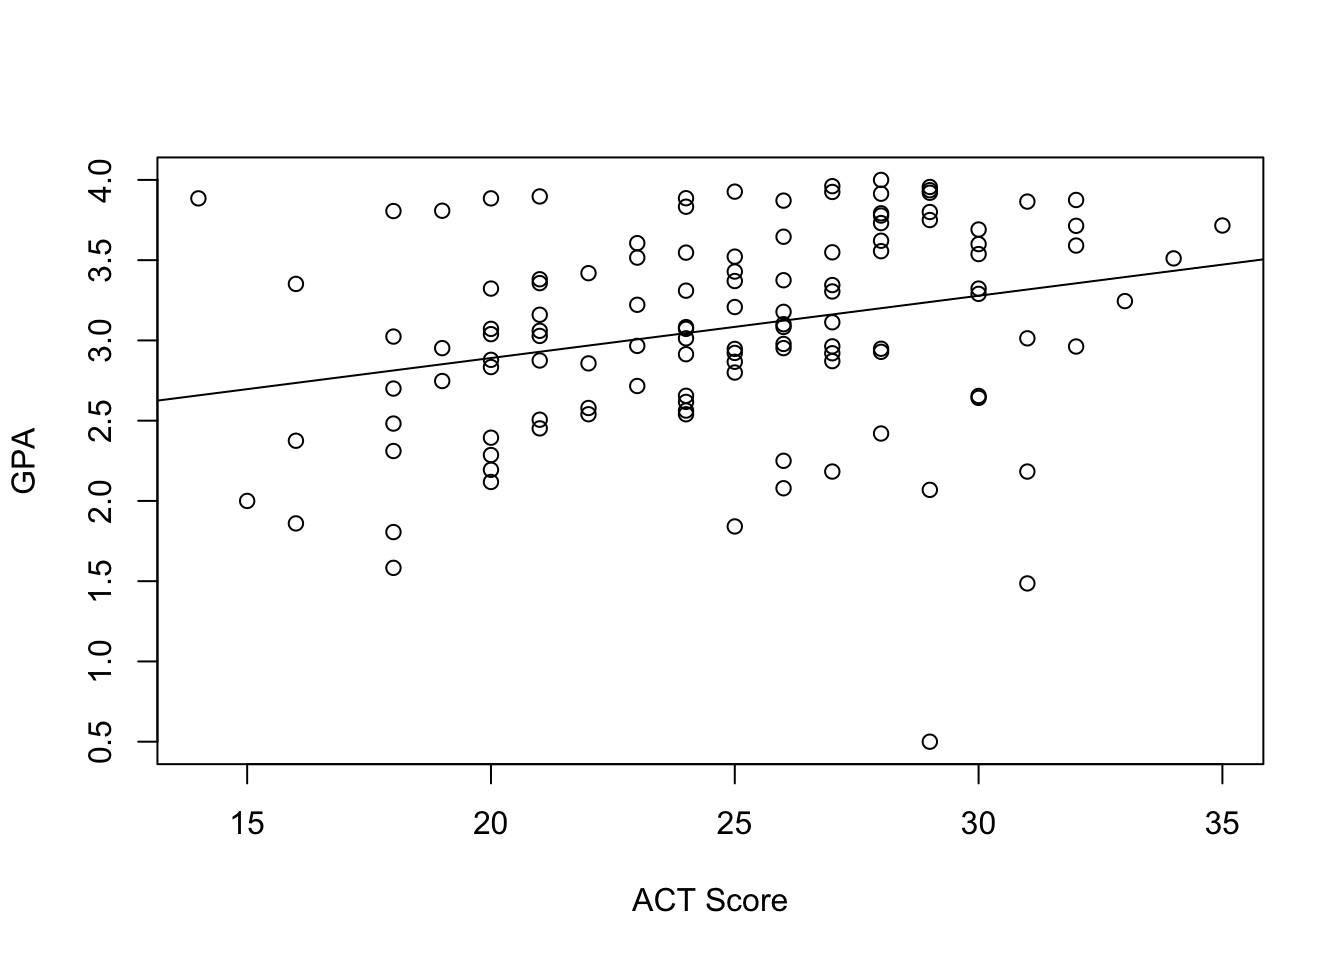
\includegraphics{CSCI-E-106-Fall-2020-Homework-1-Solutions_files/figure-latex/unnamed-chunk-2-1.pdf}
\#\#\# c) \#\#\# \_Solution: it is 3.47

\begin{Shaded}
\begin{Highlighting}[]
\NormalTok{Xnew=}\KeywordTok{data.frame}\NormalTok{(}\DataTypeTok{X=}\DecValTok{35}\NormalTok{)}
\KeywordTok{predict}\NormalTok{(f1a,Xnew)}
\end{Highlighting}
\end{Shaded}

\begin{verbatim}
##        1 
## 3.472999
\end{verbatim}

\hypertarget{d}{%
\subsubsection{d)}\label{d}}

\hypertarget{solution-0.0388}{%
\subsubsection{\_Solution: 0.0388}\label{solution-0.0388}}

\hypertarget{e}{%
\subsubsection{e)}\label{e}}

\hypertarget{solution-yes-they-do-sum-to-zero}{%
\subsubsection{\_Solution: yes they do sum to
zero}\label{solution-yes-they-do-sum-to-zero}}

\begin{Shaded}
\begin{Highlighting}[]
\NormalTok{ei=f1a}\OperatorTok{$}\NormalTok{residuals}
\KeywordTok{sum}\NormalTok{(ei)}
\end{Highlighting}
\end{Shaded}

\begin{verbatim}
## [1] -2.942091e-15
\end{verbatim}

\hypertarget{f}{%
\subsubsection{f)}\label{f}}

\hypertarget{solution-see-below-they-are-expressed-as-grade-points}{%
\subsubsection{\_Solution: see below, they are expressed as grade
points}\label{solution-see-below-they-are-expressed-as-grade-points}}

\begin{Shaded}
\begin{Highlighting}[]
\NormalTok{sigma2<-}\KeywordTok{sum}\NormalTok{(ei}\OperatorTok{^}\DecValTok{2}\NormalTok{)}\OperatorTok{/}\NormalTok{(}\DecValTok{120-2}\NormalTok{)}
\NormalTok{sigma=}\KeywordTok{sqrt}\NormalTok{(sigma2)}
\KeywordTok{cbind}\NormalTok{(sigma2,sigma)}
\end{Highlighting}
\end{Shaded}

\begin{verbatim}
##         sigma2    sigma
## [1,] 0.3882848 0.623125
\end{verbatim}

Problem 2

Typographical errors shown below are the number of galleys for a
manuscript (X) and the dollar cost of correcting typographical errors
(Y) in a random sample of recent orders handled by a firm specializing
in technical manuscripts. Assume that the regression model Yi = β1X1 +
ε\_i is appropriate, with normally distributed independent error terms
whose variance is a σ\^{}2 = 16. (20 pts)

\begin{enumerate}
\def\labelenumi{\alph{enumi})}
\item
  Evaluate the likelihood function for \(\beta_{1}= 1,2, 3,…,100\). For
  which of \(\beta_{1}\) values is the likelihood function largest?
  (10pts)
\item
  The maximum likelihood estimator is
  \(\b_{1}=\sum X_{i} Y_{i}/\sum X_{i}^2\). Find the maximum likelihood
  estimate. Are your results in part (a) consistent with this estimate?
  (10 pts)
\end{enumerate}

\hypertarget{a-1}{%
\subsubsection{a)}\label{a-1}}

\hypertarget{solution-ignoring-the-constant-part-of-the-likelihood-function-for-beta18-gives-the-maximum-likelihood.}{%
\subsubsection{\_Solution: Ignoring the constant part of the likelihood
function for beta=18 gives the maximum
likelihood.}\label{solution-ignoring-the-constant-part-of-the-likelihood-function-for-beta18-gives-the-maximum-likelihood.}}

\begin{Shaded}
\begin{Highlighting}[]
\NormalTok{y=}\KeywordTok{c}\NormalTok{(}\DecValTok{128}\NormalTok{,}\DecValTok{213}\NormalTok{,}\DecValTok{75}\NormalTok{,}\DecValTok{250}\NormalTok{,}\DecValTok{446}\NormalTok{,}\DecValTok{540}\NormalTok{)}
\NormalTok{x=}\KeywordTok{c}\NormalTok{(}\DecValTok{7}\NormalTok{,}\DecValTok{12}\NormalTok{,}\DecValTok{4}\NormalTok{,}\DecValTok{14}\NormalTok{,}\DecValTok{25}\NormalTok{,}\DecValTok{30}\NormalTok{)}
\NormalTok{beta=}\KeywordTok{seq}\NormalTok{(}\DecValTok{1}\NormalTok{,}\DecValTok{100}\NormalTok{)}

\NormalTok{prg2<-}\ControlFlowTok{function}\NormalTok{(x,y,beta)\{ }
\NormalTok{  n<-}\KeywordTok{length}\NormalTok{(beta)}
\NormalTok{  c<-((}\DecValTok{2}\OperatorTok{*}\NormalTok{pi)}\OperatorTok{^}\NormalTok{(}\OperatorTok{-}\DecValTok{3}\NormalTok{))}\OperatorTok{*}\DecValTok{4}\OperatorTok{^}\NormalTok{(}\OperatorTok{-}\DecValTok{6}\NormalTok{)}
\NormalTok{  out<-}\KeywordTok{data.frame}\NormalTok{(}\KeywordTok{matrix}\NormalTok{(}\DecValTok{0}\NormalTok{,}\DataTypeTok{nrow=}\NormalTok{n,}\DataTypeTok{ncol=}\DecValTok{2}\NormalTok{))}
  \ControlFlowTok{for}\NormalTok{ (i }\ControlFlowTok{in} \DecValTok{1}\OperatorTok{:}\NormalTok{n)\{  }
\NormalTok{    ypred=beta[i]}\OperatorTok{*}\NormalTok{x}
\NormalTok{    e=y}\OperatorTok{-}\NormalTok{ypred}
\NormalTok{    m1=(e}\OperatorTok{^}\DecValTok{2}\NormalTok{)}\OperatorTok{/}\DecValTok{16}
\NormalTok{    Li=}\KeywordTok{exp}\NormalTok{(}\OperatorTok{-}\FloatTok{0.5}\OperatorTok{*}\KeywordTok{sum}\NormalTok{(m1))}
\NormalTok{    out[i,}\DecValTok{1}\NormalTok{]<-beta[i]}
\NormalTok{    out[i,}\DecValTok{2}\NormalTok{]<-}\KeywordTok{prod}\NormalTok{(Li)}
\NormalTok{  \}    }
  \KeywordTok{dimnames}\NormalTok{(out[[}\DecValTok{2}\NormalTok{]])[[}\DecValTok{2}\NormalTok{]]}\OperatorTok{<}\KeywordTok{c}\NormalTok{(}\StringTok{"b1"}\NormalTok{,}\StringTok{"L"}\NormalTok{)    }
\NormalTok{  out}
\NormalTok{  \}}
\KeywordTok{round}\NormalTok{(}\KeywordTok{prg2}\NormalTok{(x,y,beta),}\DecValTok{5}\NormalTok{)}
\end{Highlighting}
\end{Shaded}

\begin{verbatim}
##      X1      X2
## 1     1 0.00000
## 2     2 0.00000
## 3     3 0.00000
## 4     4 0.00000
## 5     5 0.00000
## 6     6 0.00000
## 7     7 0.00000
## 8     8 0.00000
## 9     9 0.00000
## 10   10 0.00000
## 11   11 0.00000
## 12   12 0.00000
## 13   13 0.00000
## 14   14 0.00000
## 15   15 0.00000
## 16   16 0.00000
## 17   17 0.00000
## 18   18 0.26915
## 19   19 0.00000
## 20   20 0.00000
## 21   21 0.00000
## 22   22 0.00000
## 23   23 0.00000
## 24   24 0.00000
## 25   25 0.00000
## 26   26 0.00000
## 27   27 0.00000
## 28   28 0.00000
## 29   29 0.00000
## 30   30 0.00000
## 31   31 0.00000
## 32   32 0.00000
## 33   33 0.00000
## 34   34 0.00000
## 35   35 0.00000
## 36   36 0.00000
## 37   37 0.00000
## 38   38 0.00000
## 39   39 0.00000
## 40   40 0.00000
## 41   41 0.00000
## 42   42 0.00000
## 43   43 0.00000
## 44   44 0.00000
## 45   45 0.00000
## 46   46 0.00000
## 47   47 0.00000
## 48   48 0.00000
## 49   49 0.00000
## 50   50 0.00000
## 51   51 0.00000
## 52   52 0.00000
## 53   53 0.00000
## 54   54 0.00000
## 55   55 0.00000
## 56   56 0.00000
## 57   57 0.00000
## 58   58 0.00000
## 59   59 0.00000
## 60   60 0.00000
## 61   61 0.00000
## 62   62 0.00000
## 63   63 0.00000
## 64   64 0.00000
## 65   65 0.00000
## 66   66 0.00000
## 67   67 0.00000
## 68   68 0.00000
## 69   69 0.00000
## 70   70 0.00000
## 71   71 0.00000
## 72   72 0.00000
## 73   73 0.00000
## 74   74 0.00000
## 75   75 0.00000
## 76   76 0.00000
## 77   77 0.00000
## 78   78 0.00000
## 79   79 0.00000
## 80   80 0.00000
## 81   81 0.00000
## 82   82 0.00000
## 83   83 0.00000
## 84   84 0.00000
## 85   85 0.00000
## 86   86 0.00000
## 87   87 0.00000
## 88   88 0.00000
## 89   89 0.00000
## 90   90 0.00000
## 91   91 0.00000
## 92   92 0.00000
## 93   93 0.00000
## 94   94 0.00000
## 95   95 0.00000
## 96   96 0.00000
## 97   97 0.00000
## 98   98 0.00000
## 99   99 0.00000
## 100 100 0.00000
\end{verbatim}

\hypertarget{b-1}{%
\subsubsection{b)}\label{b-1}}

\hypertarget{solution-it-is-17.9285-with-rounding-it-is-18-similar-to-the-part-a.}{%
\subsubsection{\_Solution: it is 17.9285 with rounding it is 18, similar
to the part
a.}\label{solution-it-is-17.9285-with-rounding-it-is-18-similar-to-the-part-a.}}

\begin{Shaded}
\begin{Highlighting}[]
\NormalTok{f2<-}\KeywordTok{lm}\NormalTok{(y }\OperatorTok{~}\StringTok{ }\NormalTok{x }\DecValTok{-1}\NormalTok{)}
\NormalTok{f2}\OperatorTok{$}\NormalTok{coefficients}
\end{Highlighting}
\end{Shaded}

\begin{verbatim}
##       x 
## 17.9285
\end{verbatim}

Problem 3

Refer to the CDI data set. The number of active physicians in a CDI (Y)
is expected to be related to total population, number of hospital beds,
and total personal income. (30 points)

\begin{enumerate}
\def\labelenumi{\alph{enumi})}
\tightlist
\item
  Regress the number of active physicians in turn on each of the three
  predictor variables. State the estimated regression functions. (10
  points)
\item
  Plot the three estimated regression functions and data on separate
  graphs. Does a linear regression relation appear to provide a good fit
  for each of the three predictor variables? (10 points)
\item
  Calculate MSE for each of the three predictor variables. Which
  predictor variable leads to the smallest variability around the fitted
  regression line? Which variable would you use the estimate Y and why?
  (10 points) \#\#\# a) \#\#\# \_Solution: see below
\end{enumerate}

\begin{Shaded}
\begin{Highlighting}[]
\NormalTok{CDI <-}\StringTok{ }\KeywordTok{read.csv}\NormalTok{(}\StringTok{"CDI Data.csv"}\NormalTok{)}
\NormalTok{Y=CDI}\OperatorTok{$}\NormalTok{Number.of.active.physicians}
\NormalTok{X1=CDI}\OperatorTok{$}\NormalTok{Total.population}
\NormalTok{X2=CDI}\OperatorTok{$}\NormalTok{Number.of.hospital.beds}
\NormalTok{X3=CDI}\OperatorTok{$}\NormalTok{Total.personal.income}
\NormalTok{f31<-}\KeywordTok{lm}\NormalTok{(Y}\OperatorTok{~}\NormalTok{X1)}
\NormalTok{f32<-}\KeywordTok{lm}\NormalTok{(Y}\OperatorTok{~}\NormalTok{X2)}
\NormalTok{f33<-}\KeywordTok{lm}\NormalTok{(Y}\OperatorTok{~}\NormalTok{X3)}
\KeywordTok{rbind}\NormalTok{(f31}\OperatorTok{$}\NormalTok{coefficients,f32}\OperatorTok{$}\NormalTok{coefficients,f33}\OperatorTok{$}\NormalTok{coefficients)}
\end{Highlighting}
\end{Shaded}

\begin{verbatim}
##      (Intercept)          X1
## [1,]  -110.63478 0.002795425
## [2,]   -95.93218 0.743116444
## [3,]   -48.39485 0.131701189
\end{verbatim}

\hypertarget{b-2}{%
\subsubsection{b)}\label{b-2}}

\hypertarget{solution-yes-there-is-a-good-fit-for-each-of-variables.}{%
\subsubsection{\_Solution: yes, there is a good fit for each of
variables.}\label{solution-yes-there-is-a-good-fit-for-each-of-variables.}}

\begin{Shaded}
\begin{Highlighting}[]
\KeywordTok{par}\NormalTok{(}\DataTypeTok{mfrow=}\KeywordTok{c}\NormalTok{(}\DecValTok{1}\NormalTok{,}\DecValTok{3}\NormalTok{))}
\KeywordTok{plot}\NormalTok{(X1,Y,}\DataTypeTok{xlab=}\StringTok{"Total Population"}\NormalTok{,}\DataTypeTok{ylab=}\StringTok{"The number of active physicians"}\NormalTok{)}
\KeywordTok{abline}\NormalTok{(f31)}
\KeywordTok{plot}\NormalTok{(X2,Y,}\DataTypeTok{xlab=}\StringTok{"Number of hospital beds"}\NormalTok{,}\DataTypeTok{ylab=}\StringTok{"The number of active physicians"}\NormalTok{)}
\KeywordTok{abline}\NormalTok{(f32)}
\KeywordTok{plot}\NormalTok{(X3,Y,}\DataTypeTok{xlab=}\StringTok{"total personal income"}\NormalTok{,}\DataTypeTok{ylab=}\StringTok{"The number of active physicians"}\NormalTok{)}
\KeywordTok{abline}\NormalTok{(f33)}
\end{Highlighting}
\end{Shaded}

\includegraphics{CSCI-E-106-Fall-2020-Homework-1-Solutions_files/figure-latex/unnamed-chunk-9-1.pdf}
\#\#\# c) \#\#\# \_Solution: Number of Hospital beds gives the smallest
MSE. I would use this variable since it has the lowest MSE.

\begin{Shaded}
\begin{Highlighting}[]
\NormalTok{n=}\KeywordTok{dim}\NormalTok{(CDI)[}\DecValTok{1}\NormalTok{]}
\NormalTok{MSE1=}\KeywordTok{sum}\NormalTok{(f31}\OperatorTok{$}\NormalTok{residuals}\OperatorTok{^}\DecValTok{2}\NormalTok{)}\OperatorTok{/}\NormalTok{(n}\DecValTok{-2}\NormalTok{)}
\NormalTok{MSE2=}\KeywordTok{sum}\NormalTok{(f32}\OperatorTok{$}\NormalTok{residuals}\OperatorTok{^}\DecValTok{2}\NormalTok{)}\OperatorTok{/}\NormalTok{(n}\DecValTok{-2}\NormalTok{)}
\NormalTok{MSE3=}\KeywordTok{sum}\NormalTok{(f33}\OperatorTok{$}\NormalTok{residuals}\OperatorTok{^}\DecValTok{2}\NormalTok{)}\OperatorTok{/}\NormalTok{(n}\DecValTok{-2}\NormalTok{)}
\KeywordTok{cbind}\NormalTok{(MSE1,MSE2,MSE3)}
\end{Highlighting}
\end{Shaded}

\begin{verbatim}
##          MSE1     MSE2     MSE3
## [1,] 372203.5 310191.9 324539.4
\end{verbatim}

Problem 4 Refer to the CDI data set. Use the number of active physicians
as Y and total personal income as X. Select 1,000 random samples of 400
observations, fit the regression model and record β0 and β1 for each
selected sample. Calculate the mean and variance of β0 and β1 based on
the 1,000 different regression line and compare against the regression
model in question 3 part a. (20 points)

\hypertarget{solution-mean-values-bo--49.12-and-b10.1317-variances-bo75.9-b10.0000013-from-question-3-bo-48.3948489-and-b1-0.1317012.-bo-seems-off-and-b1-seems-correct-indicating-that-bo-is-not-a-reliable-estimate-will-change-significantly-sample-to-sample.}{%
\subsubsection{\_Solution: Mean values: bo= -49.12 and b1=0.1317
Variances: bo=75.9 b1=0.0000013 from question 3, bo=-48.3948489 and b1=
0.1317012. bo seems off and b1 seems correct, indicating that bo is not
a reliable estimate (will change significantly sample to
sample.)}\label{solution-mean-values-bo--49.12-and-b10.1317-variances-bo75.9-b10.0000013-from-question-3-bo-48.3948489-and-b1-0.1317012.-bo-seems-off-and-b1-seems-correct-indicating-that-bo-is-not-a-reliable-estimate-will-change-significantly-sample-to-sample.}}

\begin{Shaded}
\begin{Highlighting}[]
\NormalTok{dat<-}\KeywordTok{data.frame}\NormalTok{(}\KeywordTok{cbind}\NormalTok{(X3,Y))}
\NormalTok{prg3<-}\ControlFlowTok{function}\NormalTok{(dat)\{}
\NormalTok{  n=}\KeywordTok{dim}\NormalTok{(dat)[}\DecValTok{1}\NormalTok{]}
\NormalTok{  out<-}\KeywordTok{data.frame}\NormalTok{(}\KeywordTok{matrix}\NormalTok{(}\DecValTok{0}\NormalTok{,}\DataTypeTok{nrow=}\DecValTok{1000}\NormalTok{,}\DataTypeTok{ncol=}\DecValTok{2}\NormalTok{))}
  \ControlFlowTok{for}\NormalTok{(i }\ControlFlowTok{in} \DecValTok{1}\OperatorTok{:}\DecValTok{1000}\NormalTok{)\{}
\NormalTok{    ind=}\KeywordTok{sample}\NormalTok{(}\DecValTok{1}\OperatorTok{:}\NormalTok{n,}\DecValTok{400}\NormalTok{)}
\NormalTok{    dat1=dat[ind,]}
\NormalTok{    f<-}\KeywordTok{lm}\NormalTok{(Y}\OperatorTok{~}\NormalTok{X3,}\DataTypeTok{data=}\NormalTok{dat1)}
\NormalTok{    out[i,]<-}\KeywordTok{c}\NormalTok{(f}\OperatorTok{$}\NormalTok{coefficients)}
\NormalTok{    \}}
  \KeywordTok{dimnames}\NormalTok{(out)[[}\DecValTok{2}\NormalTok{]]<-}\KeywordTok{c}\NormalTok{(}\StringTok{"b0"}\NormalTok{,}\StringTok{"b1"}\NormalTok{)}
\NormalTok{  out}
\NormalTok{\}}
\KeywordTok{set.seed}\NormalTok{(}\DecValTok{123}\NormalTok{)}
\NormalTok{out3=}\KeywordTok{prg3}\NormalTok{(dat)}
\KeywordTok{apply}\NormalTok{(out3,}\DecValTok{2}\NormalTok{,mean)}
\end{Highlighting}
\end{Shaded}

\begin{verbatim}
##          b0          b1 
## -48.9238113   0.1317611
\end{verbatim}

\begin{Shaded}
\begin{Highlighting}[]
\KeywordTok{apply}\NormalTok{(out3,}\DecValTok{2}\NormalTok{,var)}
\end{Highlighting}
\end{Shaded}

\begin{verbatim}
##           b0           b1 
## 7.024623e+01 1.186634e-06
\end{verbatim}

\begin{Shaded}
\begin{Highlighting}[]
\NormalTok{f33}\OperatorTok{$}\NormalTok{coefficients}
\end{Highlighting}
\end{Shaded}

\begin{verbatim}
## (Intercept)          X3 
## -48.3948489   0.1317012
\end{verbatim}

\end{document}
